%% ===============================================
\begin{subfigure}[b]{0.14\textwidth}
\caption{\label{fig:sq-1nn}}
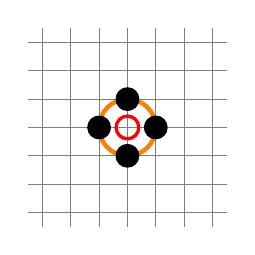
\begin{tikzpicture}[scale=0.36]
\draw[step=1,color=gray] (-3.5,-3.5) grid (3.5,3.5);
\draw[very thick,red] (0, 0) circle (.4);
\draw[ultra thick,orange] (0,0) circle (1);
\filldraw[black] (0,-1) circle (.4);
\filldraw[black] (0,+1) circle (.4);
\filldraw[black] (-1,0) circle (.4);
\filldraw[black] (+1,0) circle (.4);
\end{tikzpicture}
\end{subfigure}
%% ===============================================
\hfill
%% ===============================================
\begin{subfigure}[b]{0.14\textwidth}
\caption{\label{fig:sq-2nn}}
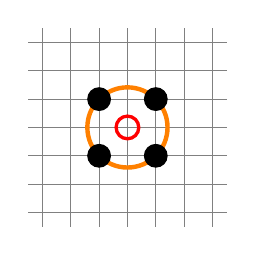
\begin{tikzpicture}[scale=0.36]
\draw[step=1,color=gray] (-3.5,-3.5) grid (3.5,3.5);
\draw[very thick,red] (0, 0) circle (.4);
\draw[ultra thick,orange] (0,0) circle (1.414213562);
\filldraw[black] (+1,-1) circle (.4);
\filldraw[black] (+1,+1) circle (.4);
\filldraw[black] (-1,-1) circle (.4);
\filldraw[black] (-1,+1) circle (.4);
\end{tikzpicture}
\end{subfigure}
%% ===============================================
\hfill
%% ===============================================
\begin{subfigure}[b]{0.14\textwidth}
\caption{\label{fig:sq-3nn}}
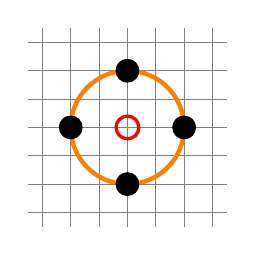
\begin{tikzpicture}[scale=0.36]
\draw[step=1,color=gray] (-3.5,-3.5) grid (3.5,3.5);
\draw[very thick,red] (0, 0) circle (.4);
\draw[ultra thick,orange] (0,0) circle (2);
\filldraw[black] ( 0,-2) circle (.4);
\filldraw[black] ( 0,+2) circle (.4);
\filldraw[black] (-2, 0) circle (.4);
\filldraw[black] (+2, 0) circle (.4);
\end{tikzpicture}
\end{subfigure}
%% ===============================================
\hfill
%% ===============================================
\begin{subfigure}[b]{0.14\textwidth}
\caption{\label{fig:sq-4nn}}
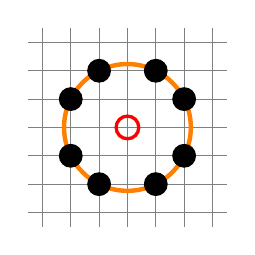
\begin{tikzpicture}[scale=0.36]
\draw[step=1,color=gray] (-3.5,-3.5) grid (3.5,3.5);
\draw[very thick,red] (0, 0) circle (.4);
\draw[ultra thick,orange] (0,0) circle (2.2360679);
\filldraw[black] (-2,-1) circle (.4);
\filldraw[black] (-2,+1) circle (.4);
\filldraw[black] (-1,-2) circle (.4);
\filldraw[black] (-1,+2) circle (.4);
\filldraw[black] (+1,-2) circle (.4);
\filldraw[black] (+1,+2) circle (.4);
\filldraw[black] (+2,-1) circle (.4);
\filldraw[black] (+2,+1) circle (.4);
\end{tikzpicture}
\end{subfigure}
%% ===============================================
\hfill
%% ===============================================
\begin{subfigure}[b]{0.14\textwidth}
\caption{\label{fig:sq-5nn}}
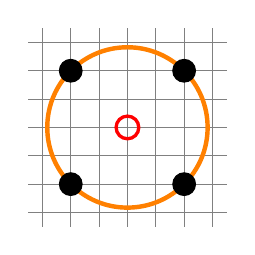
\begin{tikzpicture}[scale=0.36]
\draw[step=1,color=gray] (-3.5,-3.5) grid (3.5,3.5);
\draw[very thick,red] (0, 0) circle (.4);
\draw[ultra thick,orange] (0,0) circle (2.8284271);
\filldraw[black] (-2,-2) circle (.4);
\filldraw[black] (-2,+2) circle (.4);
\filldraw[black] (+2,-2) circle (.4);
\filldraw[black] (+2,+2) circle (.4);
\end{tikzpicture}
\end{subfigure}
%% ===============================================
\hfill
%% ===============================================
\begin{subfigure}[b]{0.14\textwidth}
\caption{\label{fig:sq-6nn}}
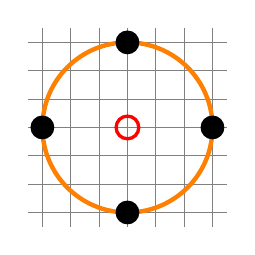
\begin{tikzpicture}[scale=0.36]
\draw[step=1,color=gray] (-3.5,-3.5) grid (3.5,3.5);
\draw[very thick,red] (0, 0) circle (.4);
\draw[ultra thick,orange] (0,0) circle (3);
\filldraw[black] (0,-3) circle (.4);
\filldraw[black] (0,+3) circle (.4);
\filldraw[black] (-3,0) circle (.4);
\filldraw[black] (+3,0) circle (.4);
\end{tikzpicture}
\end{subfigure}
%% ===============================================